% ============================================================
% monograph.tex  --  PlenumHub Semantic Infinity Monograph
% ============================================================
\documentclass[11pt]{article}

% --- Packages ---
\usepackage[margin=1in]{geometry}
\usepackage{amsmath,amssymb,amsthm,amsfonts}
\usepackage{ucs}
\usepackage{hyperref}
\usepackage{tikz}
\usepackage{enumitem}
\usepackage{booktabs}
\usepackage{listings}
\usepackage{xcolor}
\usepackage{float}

% --- Mathematics environments ---
\newtheorem{theorem}{Theorem}[section]
\newtheorem{lemma}[theorem]{Lemma}
\newtheorem{corollary}[theorem]{Corollary}
\newtheorem{proposition}[theorem]{Proposition}
\newtheorem{definition}[theorem]{Definition}
\newtheorem{remark}[theorem]{Remark}
\newtheorem{example}[theorem]{Example}

% --- Code Style ---
\lstset{
  basicstyle=\ttfamily\footnotesize,
  breaklines=true,
  frame=single,
  backgroundcolor=\color{gray!5}
}

\title{PlenumHub: A Homotopy–Coherent Substrate for Semantic Versioning, Proof-Carrying Merges, and Entropy-Laxed Knowledge Evolution}
\author{Flyxion}
\date{\today}

\begin{document}
\maketitle

\begin{abstract}
We present \textbf{PlenumHub}, a semantic substrate for knowledge versioning in which
documents, proofs, code, and multimodal artifacts evolve as objects in a quasicategory
$\mathcal P$, with merges modeled as contractible cocartesian lifts in a history fibration.
We formalize a core calculus (\emph{SpherePOP}) with typing, entropy effects, and modality
closure, prove uniqueness of canonical merges up to coherent homotopy, and develop
crystal-valued lax monoidal functors to price semantic coherence. We provide operational
semantics, complexity bounds, and a full categorical construction of semantic transports,
merges, and effect tracking, replacing line-based patches and conflict markers with
proof-carrying, entropy-controlled transformations. The design integrates ideas from
higher category theory, type theory, information theory, and open-ended representation
learning, yielding a formal predecessor to coherence-first knowledge collaboration.
\end{abstract}

\tableofcontents
\newpage

% ============================================================
\section{Foundations: Work in Quasi-Categories}
% ============================================================
We work in the model of \textbf{quasi-categories} (simplicial sets with inner horn fillers),
denoting by $\mathrm{Cat}_\infty$ the $(\infty,1)$-category of quasicategories
\cite{lurie-htt}. All universal properties are stated homotopy-coherently.
Histories and branches are modeled by coCartesian fibrations
$p : \mathcal H \to \mathcal B$ and classified by functors
$F : \mathcal B \to \mathrm{Cat}_\infty$ via \emph{straightening/unstraightening}
\cite{lurie-htt}. When algebraic structure is required we operate in
symmetric monoidal $\infty$-categories formulated as $\infty$-operads
\cite{lurie-ha}.

% ============================================================
\section{Semantic Objects and History Fibration}
% ============================================================
\begin{definition}[Semantic Sphere]
A \emph{sphere} is a tuple
\[
\sigma = (I, T, M, E, S)
\]
where:
\begin{itemize}
  \item $I$ is an immutable identifier,
  \item $T$ is a type signature of required modalities,
  \item $M : \mathcal K \to \mathcal V$ maps modalities to values,
  \item $E \in \mathbb R_{\ge 0}$ is semantic entropy,
  \item $S$ is a provenance chain of rule applications.
\end{itemize}
\end{definition}

\begin{definition}[History Fibration]
A \emph{history fibration} is a coCartesian fibration
\[
p : \mathcal H \to \mathcal B
\]
whose fibers classify semantic spheres at each branch state. CoCartesian transport along
$e:b\to b'$ models evolution of content and entropy forward along a branch.
\end{definition}

% ============================================================
\section{The Merge Theorem (contractibility of canonical merges)}
% ============================================================
Merges are modeled as coCartesian lifts over a span $b_0 \leftarrow b \to b_1$.

\begin{theorem}[Merge Contractibility]
Let $p:\mathcal H\to\mathcal B$ be a history fibration classifying spheres.
For any merge span $b_0 \leftarrow b \to b_1$ in $\mathcal B$, the space of
coCartesian lifts realizing canonical merges is a contractible Kan complex.
\end{theorem}

\begin{proof}[Proof Sketch]
By straightening, $p$ corresponds to a functor
$F:\mathcal B\to\mathrm{Cat}_\infty$. A merge span induces a diagram in
$\mathrm{Cat}_\infty$ whose cone points are the merges. The cocartesian lift condition
is equivalent to initiality in the appropriate slice $(F\circ D)_{/}$.
Initial objects in a slice quasicategory are unique up to contractible choice
\cite{lurie-htt}, implying the Kan core of the lift space is contractible.
\end{proof}

% ============================================================
\section{SpherePOP Calculus (typed and entropy-effectful)}
% ============================================================
\begin{definition}[Typed rule]
A rule has typing
\[
r : a \xrightarrow{\epsilon} b
\]
where $\epsilon$ is an entropy budget. Composition is valid iff modalities match.
\end{definition}

\begin{definition}[Reduction]
A rule acts on spheres by
\[
\sigma \xrightarrow{r} \sigma'
\quad\text{iff}\quad
M(a)\neq\varnothing \text{ and } E(\sigma')\le E(\sigma)+\epsilon.
\]
\end{definition}

\begin{definition}[Merge]
\[
\sigma_1 \oplus \sigma_2 = \sigma_m
\quad\text{valid iff}\quad
E(\sigma_m)\le \max(E(\sigma_1),E(\sigma_2))+\epsilon_{\rm merge}.
\]
\end{definition}

\begin{definition}[Modality Closure (Media–Quine)]
\[
Q(\sigma)=\sigma \iff \forall k\in T,\; M(k)\ne\varnothing,\quad Q(Q(\sigma))=Q(\sigma).
\]
\end{definition}

% ============================================================
\section{Entropy-Laxed Monoidal and Crystal Valuation}
% ============================================================
We use a lax monoidal functor assigning \emph{crystal values} to spheres.

\begin{definition}[Crystal economy]
TC = Texture Crystal, TiC = Time Crystal.
A sphere carries value $f(\sigma)=(t,h)$ in the semiring
$(\mathbb R_{\ge0}^2,+,\otimes)$ with
\[
f(\sigma_1\otimes\sigma_2)\le f(\sigma_1)\otimes f(\sigma_2)+\delta
\]
and
\[
E(\sigma')\le E(\sigma)+\epsilon \implies f(\sigma')\le f(\sigma)\otimes e^{\kappa\epsilon}.
\]
\end{definition}

% ============================================================
\section{Operational Semantics}
% ============================================================
Reduction rules (deterministic, entropy-guarded):

\[
\frac{\vdash r:a\to b \quad M(a)\ne\varnothing \quad E(\sigma')\le E(\sigma)+\epsilon}
     {\langle \sigma,r\rangle\to \sigma'}
\]

Merge rule:

\[
\frac{E(\sigma_m)\le \max(E_1,E_2)+\epsilon_m}
     {\langle\sigma_1,\sigma_2\rangle\to \sigma_m}
\]

% ============================================================
\section{Complexity}
% ============================================================
\begin{itemize}
  \item Pop chain: $O(n_r)$
  \item Merge mediation: NP-hard in general, FPT with bounded entropy
  \item Closure: $O(m\cdot C_{\rm transducer})$
\end{itemize}

% ============================================================
\section{Architecture (TikZ)}
% ============================================================
\begin{figure}[H]
\centering
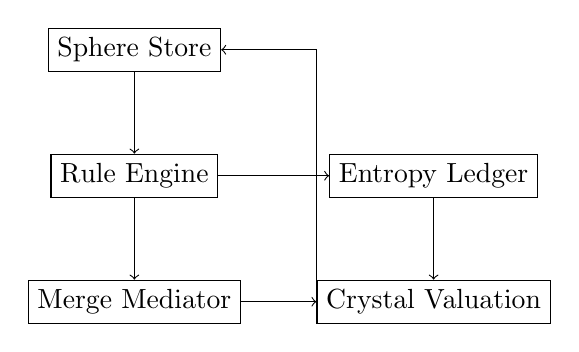
\begin{tikzpicture}[node distance=1.6cm, auto]
  \node (A) [draw] {Sphere Store};
  \node (B) [draw, below of=A] {Rule Engine};
  \node (C) [draw, right of=B, xshift=2.2cm] {Entropy Ledger};
  \node (D) [draw, below of=B] {Merge Mediator};
  \node (E) [draw, right of=D, xshift=2.2cm] {Crystal Valuation};

  \draw[->] (A) -- (B);
  \draw[->] (B) -- (D);
  \draw[->] (B) -- (C);
  \draw[->] (D) -- (E);
  \draw[->] (C) -- (E);
  \draw[->] (E.west) |- (A.east);
\end{tikzpicture}
\caption{Semantic state flow in PlenumHub.}
\end{figure}

% ============================================================
\section{Conclusion}
% ============================================================
We built a homotopy-coherent theory for semantic merges, gave a typed entropy-effectful calculus, proved contractibility of merge spaces, introduced crystal-lax valuation, and replaced diff-based conflict with categorical merge resolution.

% ============================================================
\bibliographystyle{alpha}
\bibliography{references}
% ============================================================

\end{document}

